\documentclass[a4paper]{article}
\usepackage[a4paper,top=3cm,bottom=2cm,left=3cm,right=3cm,marginparwidth=1.75cm]{geometry}
\usepackage[english]{babel}
\usepackage[utf8x]{inputenc}
\usepackage{amsmath}
\usepackage{graphicx}

% Macro shortcuts
\newcommand{\mb}[1]{{\mathbf{#1}}}
\newcommand{\II}{\mb{I}}
\newcommand{\PP}{\mb{P}}
\newcommand{\uu}{\mb{u}}
\newcommand{\eepsilon}{\boldsymbol{\epsilon}}

\title{Stretch Bar}
\author{Xuchen Han }
\date{February 2021}

\begin{document}
\maketitle
\section{Problem Setup}

\begin{figure}[!h]
  \centering
  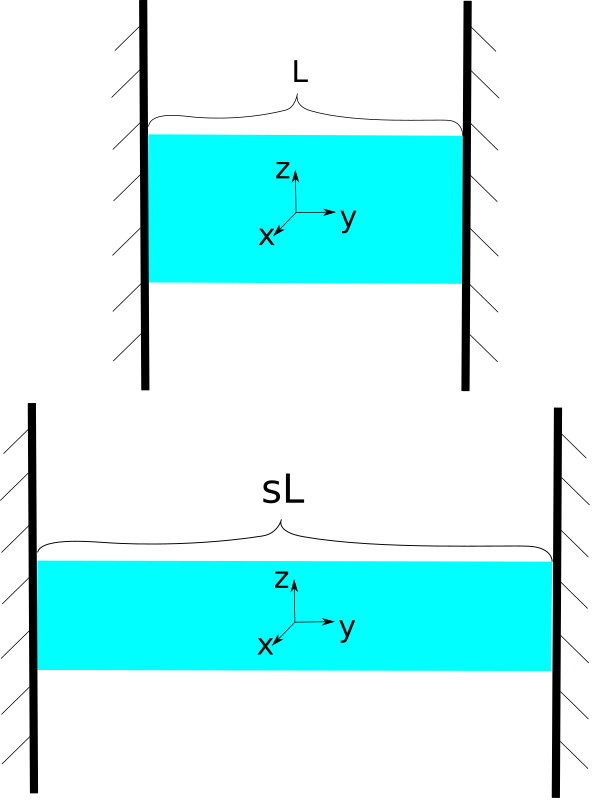
\includegraphics[width=0.5\columnwidth]{stretch_bar.png}
  \caption{\label{fig:problem}
    Problem description.}
\end{figure}

We consider an elastic block stretched on the side by Dirichlet boundary
conditions. The bar occupies the domain $[-\frac{Lx}{2}, \frac{Lx}{2}]
\times [-\frac{Ly}{2}, \frac{Ly}{2}] \times [-\frac{Lz}{2}, \frac{Lz}{2}]$.
We assume linear elasticity with Young's modulus $E$ and Poisson ratio $\nu$.
We apply Dirichlet boundary condition at $y = \frac{L}{2}$ and
$y = -\frac{L}{2}$ so that the bar is stretched by a factor of $s = 1+\epsilon$
in the $y$-direction. In other words, the boundary condition applied on the
displacement $\uu = (u_1(x,y,z), u_2(x,y,z), u_3(x,y,z))^T$ takes the form
\begin{align*}
  u_2(x,-\frac{L}{2},z) = -\frac{\epsilon L}{2} \\
  u_2(x,\frac{L}{2},z) = \frac{\epsilon L}{2}.
\end{align*}
We use the symmetry of the problem and restrict our attention to a quarter of
the original domain $[0, \frac{Lx}{2}] \times [-\frac{Ly}{2}, \frac{Ly}{2}]
\times [0, \frac{Lz}{2}]$ and add boundary conditions
\begin{align*}
  u_1(0,y,z) = 0, \\
  u_3(x,y,0) = 0,
\end{align*}
All other boundaries assume zero Neumann (no stress) boundary conditions.
We assume zero gravity for simplicity.

\section{Solution}
We use $\uu = (u_1(x,y,z), u_2(x,y,z), u_3(x,y,z))^T$ to denote displacement,
$\PP(x,y,z)$ to denote first Piola-Kirchhoff stress density, $\eepsilon$ to
denote the infinitesimal strain $\left(\epsilon_{ij} = \frac{1}{2}
    (\frac{\partial u_i}{\partial X_j} + \frac{\partial u_j}{\partial
      X_i})\right)$.
There is no external force as we assume zero gravity.

Under the stretching boundary condition, the bar should experience constant
uni-axial stress. Therefore, we guess the stress has the form
\begin{align*}
  \PP
  =
  \begin{bmatrix}
    0 & 0 & 0 \\
    0 & \sigma & 0 \\
    0 & 0 & 0
  \end{bmatrix}.
\end{align*}
In other words, the stress has a constant $2-2$ component and zeros everywhere
else.
With this guess, the static equilibrium equation
\begin{align*}
  \nabla \cdot \PP = 0
\end{align*}
is obviously satisfied.
We then plug this guess into the constitutive model
\begin{align*}
  \PP = 2\mu \eepsilon + \lambda \text{tr}(\eepsilon) \II,
\end{align*}
where $\mu$ and $\lambda$ are the Lame parameters related to $E$ and $\nu$ via
\begin{align}
   & \mu = \frac{E}{2(1+\nu)},\label{eq:lame1}               \\
   & \lambda = \frac{E\nu}{(1+\nu)(1-2\nu)}\label{eq:lame2},
\end{align}
and get the following equations on the diagonal:
\begin{align}
  P_{11} & = 2\mu\epsilon_{11} + \lambda(\epsilon_{11} + \epsilon_{22} +
  \epsilon_{33}) = 0 \label{eq:P11},                                     \\
  P_{22} & = 2\mu\epsilon_{22} + \lambda(\epsilon_{11} + \epsilon_{22} +
  \epsilon_{33}) = \sigma \label{eq:P22},                                \\
  P_{33} & = 2\mu\epsilon_{33} + \lambda(\epsilon_{11} + \epsilon_{22} +
  \epsilon_{33}) = 0\label{eq:P33},
\end{align}
and the following equations on the off-diagonal:
\begin{align}
  \frac{P_{12}}{2\mu} & = \epsilon_{12} = \epsilon_{21} = 0,
  \label{eq:P12}                                             \\
  \frac{P_{13}}{2\mu} & = \epsilon_{13} = \epsilon_{31} = 0,
  \label{eq:P13}                                             \\
  \frac{P_{23}}{2\mu} & = \epsilon_{23} = \epsilon_{32} = 0.
  \label{eq:P23}
\end{align}
Solving equations \eqref{eq:P11} through \eqref{eq:P33}, and utilizing the
identity in \eqref{eq:lame1} and \eqref{eq:lame2}, we get
\begin{align}
  \epsilon_{22} & = \frac{\sigma}{E}\label{eq:e22},                       \\
  \epsilon_{11} & = \epsilon_{33} = \frac{-\nu \sigma}{E}. \label{eq:e11}
\end{align}
Integrating equations \eqref{eq:e22} and \eqref{eq:e11}, we get
\begin{align}
  u_1(x,y,z) & = \frac{-\nu \sigma}{E}x + h_1(y,z), \label{eq:u1} \\
  u_2(x,y,z) & = \frac{\sigma}{E}y + h_2(x,z), \label{eq:u2}      \\
  u_3(x,y,z) & = \frac{-\nu \sigma}{E}z + h_3(x,y), \label{eq:u3}
\end{align}
where $h_1, h_2, h_3$ are arbitrary functions resulting from integration.
Using boundary conditions $u_2(x,\frac{L}{2},z) =\frac{\epsilon L}{2}$ and
$u_2(x,-\frac{L}{2},z) = -\frac{\epsilon L}{2}$, we get
\begin{align*}
  h_2(x,z) = 0, \\
  \sigma = \epsilon E.
\end{align*}
Using boundary conditions $u_1(0,y,z) = 0$ and $u_3(x,y,0) = 0$, we get
\begin{align*}
  h_1(y, z) = 0, \\
  h_3(x, y) = 0.
\end{align*}
Therefore, the final displacement is given by:
\begin{align*}
  u_1(x,y,z) & = -\nu \epsilon x, \\
  u_2(x,y,z) & = \epsilon y,      \\
  u_3(x,y,z) & = -\nu \epsilon z.
\end{align*}
We easily verify the displacement above satisfies equations \eqref{eq:P12}
through \eqref{eq:P23}.
\end{document}
